\documentclass[aspectratio=169,10pt]{beamer}
\usepackage[T1]{fontenc}
\usepackage{lmodern,amsmath,amssymb,bm,booktabs,array,graphicx,tikz}
\usetikzlibrary{arrows.meta,positioning,calc,fit}
\definecolor{navy}{HTML}{18334D}
\definecolor{blue}{HTML}{35577F}
\definecolor{teal}{HTML}{158371}
\definecolor{orange}{HTML}{DF9008}
\definecolor{muted}{HTML}{536473}
\definecolor{pale}{HTML}{EFF4F7}
\definecolor{paleteal}{HTML}{E9F5F1}
\setbeamercolor{normal text}{fg=navy,bg=white}
\setbeamercolor{structure}{fg=teal}
\setbeamercolor{frametitle}{fg=navy}
\setbeamercolor{block title}{fg=navy,bg=pale}
\setbeamercolor{block body}{fg=navy,bg=pale!65}
\setbeamercolor{alerted text}{fg=orange}
\setbeamerfont{frametitle}{size=\large,series=\bfseries}
\setbeamersize{text margin left=7mm,text margin right=7mm}
\setbeamertemplate{navigation symbols}{}
\setbeamertemplate{itemize item}{\color{teal}\small$\bullet$}
\setbeamertemplate{frametitle}{\vspace{2mm}\insertframetitle\par\vspace{1.5mm}\textcolor{teal}{\rule{\textwidth}{0.65pt}}\vspace{-2mm}}
\setbeamertemplate{footline}{\leavevmode\hbox{\begin{beamercolorbox}[wd=.80\paperwidth,ht=2.6ex,dp=1.2ex,leftskip=7mm]{normal text}\scriptsize\color{muted}PassengerAn\quad\textbar\quad Symmetry-guided SPRING\quad\textbar\quad 16 November 2026\end{beamercolorbox}\begin{beamercolorbox}[wd=.20\paperwidth,ht=2.6ex,dp=1.2ex,rightskip=7mm plus1fil]{normal text}\hfill\scriptsize\color{muted}\insertframenumber\,/\,\inserttotalframenumber\end{beamercolorbox}}}
\setlength{\abovedisplayskip}{5pt}
\setlength{\belowdisplayskip}{5pt}
\setlength{\tabcolsep}{5pt}
\hypersetup{colorlinks=true,urlcolor=teal,linkcolor=teal,pdftitle={Symmetry-guided SPRING on the Haldane sphere},pdfauthor={PassengerAn}}
\pdfstringdefDisableCommands{\def\translate#1{#1}}
\graphicspath{{support/figures/}}
\newcommand{\src}[1]{\vfill{\fontsize{6.3}{7.5}\selectfont\color{muted}#1\par}}
\newcommand{\take}[1]{\vspace{1mm}\begin{beamercolorbox}[sep=1.6mm,wd=\textwidth]{block body}\small\color{teal}\textbf{#1}\end{beamercolorbox}}
\newcommand{\E}{\mathbb E}
\newcommand{\R}{\mathbb R}
\newcommand{\ket}[1]{\lvert #1\rangle}
\newcommand{\bra}[1]{\langle #1\rvert}
\newcommand{\nn}{\mathbf n}
\newcommand{\fidelity}{\mathcal F}
\newcolumntype{L}[1]{>{\raggedright\arraybackslash}p{#1}}
\title{Symmetry-guided SPRING on the Haldane sphere}
\author{PassengerAn}
\date{16 November 2026}
\begin{document}

% 1
\begin{frame}[plain]
\vspace{5mm}
{\color{teal}\small NEURAL QUANTUM STATES\quad / \quad CONSERVED-OPERATOR EVOLUTION}\par
\vspace{5mm}
{\fontsize{27}{32}\selectfont\bfseries Symmetry-guided SPRING\\on the Haldane sphere}\par
\vspace{4mm}
{\large From energy minimization to an $L^2$-augmented update}\par
\vspace{6mm}
\begin{columns}[T,onlytextwidth]
\column{.31\textwidth}\textbf{Physics}\par\small LLL occupation basis and rotationally invariant pseudopotentials.
\column{.31\textwidth}\textbf{Method}\par\small SPRING direction memory with a conserved-operator force.
\column{.31\textwidth}\textbf{Evidence}\par\small Matched short control, long continuation, and exact frozen-state checks.
\end{columns}
\vfill
{\small PassengerAn\quad\textbar\quad 16 November 2026}\par
{\scriptsize\color{muted}20 main slides + 5 technical/reference slides. Saved numerical calculations; no new training for this update.}
\end{frame}

\section{Physical model and neural representation}
% 2
\begin{frame}{Haldane sphere: finite LLL space with rotational symmetry}
\begin{columns}[T,onlytextwidth]
\column{.46\textwidth}
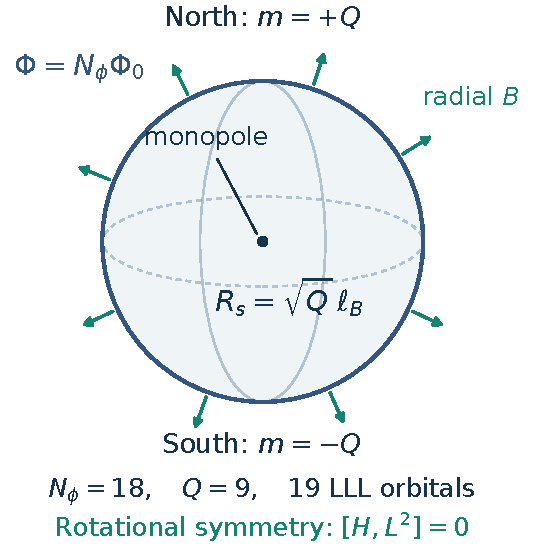
\includegraphics[width=\linewidth,height=4.7cm,keepaspectratio]{haldane_sphere_symmetry.pdf}
\column{.51\textwidth}
\begin{itemize}\setlength\itemsep{5pt}
\item Flux $N_\phi=2Q$; LLL orbitals have $\ell=Q$, $m=-Q,\ldots,Q$.
\item At the $1/3$ Laughlin shift,
\[
N_\phi=3(N_e-1).
\]
\item Here $N_e=7$, $Q=9$: \textbf{19 LLL orbitals}.
\item A rotationally invariant interaction satisfies
\[
[H,L^2]=[H,L_z]=0.
\]
\item Landau-level mixing is neglected; kinetic energy is a constant.
\end{itemize}
\end{columns}
\take{The sphere supplies a conserved angular momentum without imposing a particular total $L$ on the neural state.}
\src{Haldane, PRL 51, 605 (1983) [1]. Fractional filling and the flux shift alone do not establish a topological phase.}
\end{frame}

% 3
\begin{frame}{Occupation inputs preserve antisymmetry and $L_z$, not total $L$}
\[
\ket{\nn}=(c^\dagger_{-9})^{n_{-9}}\cdots(c^\dagger_9)^{n_9}\ket0,
\qquad
\ket{\Psi_\theta}=\sum_{\nn\in\mathcal B_{7,0}}\psi_\theta(\nn)\ket{\nn}.
\]
\begin{columns}[T,onlytextwidth]
\column{.56\textwidth}
\begin{itemize}\setlength\itemsep{6pt}
\item Input: $\nn=(n_{-9},\ldots,n_9)\in\{0,1\}^{19}$.
\item Fix $\sum_m n_m=7$, $\sum_m mn_m=M=0$.
\item Canonical creation-operator order enforces fermionic antisymmetry.
\item The $M=0$ sector contains \textbf{1,656 configurations}.
\end{itemize}
\column{.40\textwidth}
\begin{block}{Why another operator helps}
A configuration is not generally an $L^2$ eigenstate. Sampling $M=0$ still permits coherent weight in many total-$L$ sectors.\par\medskip
$L^2$ must act on amplitudes of connected configurations; it is not a label attached to one occupation row.
\end{block}
\end{columns}
\take{The trainable output is one complex many-electron coefficient, not an orbital wavefunction.}
\src{physics.py and learned\_sector\_operators.py. No dense angular projector or ED coefficient is supplied during current training.}
\end{frame}

% 4
\begin{frame}{Use one Hamiltonian for the constraint comparison}
\small
\[
H=\sum_{i<j}\sum_{R\ {\rm odd}}V_R\,\mathcal P^{(R)}_{ij},
\qquad L_{ij}=2Q-R.
\]
\[
\boxed{\ h\equiv H/V_1=\sum_{i<j}
\left(\mathcal P^{(1)}_{ij}+0.8\mathcal P^{(3)}_{ij}+0.6\mathcal P^{(5)}_{ij}\right)\ }
\]
\begin{columns}[T,onlytextwidth]
\column{.49\textwidth}
\begin{block}{Current benchmark}
\small
All current constraint comparisons use this mixed-pseudopotential $h$.\par\medskip
ED in $N_e=7,M=0$ gives a unique $L=0$ ground state:
\[
E_0/V_1=6.2447682602.
\]
\end{block}
\column{.47\textwidth}
\begin{block}{Distinguish the parent-Hamiltonian test}
\small
The earlier pure-$V_1$ model has a zero-energy Laughlin ground state at this flux.\par\medskip
The mixed-model ED target is different. Its neural ED fidelity must not be called Laughlin fidelity.
\end{block}
\end{columns}
\take{There is no confining potential in either arm of the current comparison.}
\src{pseudopotential\_v5\_operator.py; frozen mixed-H ED eigensystem (same target throughout the comparisons). Latest NN squared overlap with the original Laughlin state is 0.377\%, versus 77.817\% with the mixed-H ED ground state.}
\end{frame}

% 5
\begin{frame}{Physical energy: coefficients in, Hamiltonian expectation out}
\[
E_H(\theta)=\frac{\bra{\Psi_\theta}H\ket{\Psi_\theta}}
{\langle\Psi_\theta|\Psi_\theta\rangle}
=\E_{p_\theta}[E_{\rm loc}(\nn)],
\qquad p_\theta(\nn)\propto|\psi_\theta(\nn)|^2,
\]
\[
E_{\rm loc}(\nn)=\sum_{\nn'}H_{\nn\nn'}\,
\frac{\psi_\theta(\nn')}{\psi_\theta(\nn)}.
\]
\begin{columns}[T,onlytextwidth]
\column{.48\textwidth}
\begin{block}{Physics operation}
Known pair-hopping matrix elements connect occupation arrays; fermionic signs are included.\par\medskip
The neural network supplies the coefficient ratios.
\end{block}
\column{.48\textwidth}
\begin{block}{ML operation}
Differentiate a scalar variational objective with respect to weights and biases.\par\medskip
Sampling estimates the objective; ED is an independent validation reference.
\end{block}
\end{columns}
\take{VMC is an estimation framework. SGD, MinSR and SPRING are optimizer choices inside it.}
\src{Carleo--Troyer [3]; SPRING [5]. The latest sampler uses importance-weighted uniform-sector proposals, rather than direct Born draws; the exact energy identity remains the same.}
\end{frame}

\section{SPRING and the conserved-operator extension}
% 6
\begin{frame}{SGD, SR and MinSR use the same physical objective}
\small Center the complex score $O_{ij}=\partial_{\theta_j}\log\psi_\theta(\nn_i)$ and local energy. For Born-quadrature weights $w_i\propto\widetilde w_i|\psi_\theta(\nn_i)|^2$, normalized to sum one,
\[
A=\begin{pmatrix}\Re(\sqrt w\,\delta O)\\ \Im(\sqrt w\,\delta O)\end{pmatrix},
\quad
e_H=\begin{pmatrix}\Re(\sqrt w\,\delta E_{\rm loc})\\ \Im(\sqrt w\,\delta E_{\rm loc})\end{pmatrix},
\quad S=A^TA,\quad f_H=A^Te_H.
\]
\renewcommand{\arraystretch}{1.35}
\begin{tabular}{@{}L{.14\textwidth}L{.46\textwidth}L{.31\textwidth}@{}}
\toprule
Method & Positive-force direction & Interpretation\\\midrule
SGD & $d=2f_H\simeq\nabla E_H$ & Euclidean parameter descent\\
SR & $d=(S+\delta I)^{-1}f_H$ & Geometric preconditioning\\
MinSR & $d=A^T(AA^T+\delta I)^{-1}e_H$ & Solve in sample space\\\bottomrule
\end{tabular}
\take{We use $\delta$ for numerical damping; $\lambda$ below denotes a physical constraint weight.}
\src{Chen--Heyl [4]; Goldshlager--Abrahamsen--Lin [5]. Real parameters, complex amplitudes; apply positive-force directions with a minus sign. Finite-batch estimators need not equal full-state gradients.}
\end{frame}

% 7
\begin{frame}{SPRING retains information from earlier sampled directions}
\[
\boxed{d_k=\mu d_{k-1}
+A_k^T(A_kA_k^T+\delta I)^{-1}
\left(e_{H,k}-A_k\mu d_{k-1}\right)}
\]
\begin{columns}[T,onlytextwidth]
\column{.53\textwidth}
\begin{enumerate}\setlength\itemsep{7pt}
\item Carry a decayed direction $\mu d_{k-1}$.
\item Measure its mismatch on the current batch.
\item Correct the observed component.
\end{enumerate}
\small $\mu=0$ recovers damped MinSR.
\column{.43\textwidth}
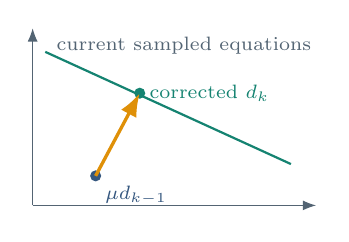
\begin{tikzpicture}[x=.8cm,y=.75cm,>=Latex]
\draw[->,muted] (0,0)--(4.5,0);
\draw[->,muted] (0,0)--(0,3);
\draw[teal,thick] (.2,2.6)--(4.1,.7);
\fill[blue] (1,.5) circle(2pt) node[below right]{\scriptsize $\mu d_{k-1}$};
\fill[teal] (1.7,1.9) circle(2pt) node[right]{\scriptsize corrected $d_k$};
\draw[->,orange,very thick] (1,.5)--(1.7,1.9);
\node[muted] at (2.4,2.7) {\scriptsize current sampled equations};
\end{tikzpicture}
\end{columns}
\[
\Delta\theta_k=-\alpha_k d_k,\qquad
\alpha_k\leq\min\!\left(\eta,\frac{\sqrt{C_{\rm cap}}}{\|d_k\|}\right).
\]
\take{Direction memory addresses discarded batch information; it does not guarantee convergence of a changing nonlinear problem.}
\src{Original SPRING: arXiv:2401.10190 [5], not the FQH/FNN paper arXiv:2412.00618 [6]. Molecular SPRING--MinSR/KFAC results are literature evidence, not a new FQHE optimizer comparison.}
\end{frame}

% 8
\begin{frame}{Modify the target evolution with a conserved operator}
\small For Hermitian $H,C$, define the normalized imaginary-time target
\[
\ket{\Psi'}\propto e^{-\tau_H H-\tau_C C}\ket{\Psi_\theta}
=e^{-\tau_H(H+\lambda C)}\ket{\Psi_\theta},
\qquad \lambda=\tau_C/\tau_H .
\]
\[
\delta\ket{\Psi}
=-\tau_H(H-E_H)\ket{\Psi}
-\tau_C(C-\langle C\rangle)\ket{\Psi}
+O(\tau^2).
\]
\begin{columns}[T,onlytextwidth]
\column{.49\textwidth}
\begin{block}{Current dimensionless choice}
\[
h=H/V_1,\qquad K=L^2/\hbar^2,
\]
\[
h_\kappa=h+\kappa K,\qquad
\kappa=\tau_K/\tau_h=0.1.
\]
\end{block}
\column{.47\textwidth}
\begin{block}{Physical role}
\small $K\geq0$ suppresses total-$L>0$ weight relative to $L=0$.\par\medskip
It is an explicit sector preference, without an exact projection or ED coefficients.
\end{block}
\end{columns}
\take{The extra force changes the evolution target; the reported physical observable remains $E_H$.}
\src{First-order normalized-state expansion. If $[H,C]=0$, the propagator factorizes exactly. The implemented neural update is a damped finite-step approximation with additional head training (slide 11).}
\end{frame}

% 9
\begin{frame}{The modified SPRING right-hand side contains both residuals}
\[
C_{\rm loc}(\nn)=\frac{(C\Psi_\theta)(\nn)}{\psi_\theta(\nn)},\qquad
e_C=\operatorname{realify}\!\left[\sqrt w(C_{\rm loc}-\langle C\rangle)\right].
\]
\[
\boxed{
d_k=\mu d_{k-1}+A_k^T(A_kA_k^T+\delta I)^{-1}
\left(e_{H,k}+\lambda e_{C,k}-A_k\mu d_{k-1}\right)}
\]
\[
\Delta\theta=-\alpha d_k,\qquad
(S+\delta I)d_k=f_H+\lambda f_C+\delta\mu d_{k-1}.
\]
\begin{itemize}\setlength\itemsep{6pt}
\item Current units: $e_h+\kappa e_K$; for physical $C=K$, $\lambda=\kappa V_1$.
\item $\lambda=0$ recovers the original energy-only right-hand side.
\item In the single-state idealization, $\lambda=\tau_C/\tau_H$ controls relative evolution.
\end{itemize}
\take{Changing the right-hand side is different from increasing batch size or numerical damping $\delta$.}
\src{Ideal centered-score formulation. For the latest augmented neural model, use the exact differentiated sampled loss and augmented metric on slide 11; finite-batch autodiff is not replaced by a naive local-residual plug-in.}
\end{frame}

% 10
\begin{frame}{Evaluate $L^2$ through a positive coherent ladder action}
\[
K=\frac{L^2}{\hbar^2}
=\frac{L_-L_+}{\hbar^2}\quad(M=0),\qquad
\langle K\rangle_\theta
=\frac{\| (L_+/\hbar)\Psi_\theta\|^2}{\|\Psi_\theta\|^2}.
\]
\[
\left[(L_+/\hbar)\Psi_\theta\right](\nn_+)
=\sum_{\nn:\,M=0}\langle\nn_+|L_+/\hbar|\nn\rangle\psi_\theta(\nn),
\qquad \nn_+:\ M=1.
\]
\begin{columns}[T,onlytextwidth]
\column{.49\textwidth}
\begin{block}{Sampling operation}
Sample $M=1$ output configurations, enumerate every incoming $M=0$ parent, then square the coherent sum.\par\smallskip
Current dimensions: $D_0=1,656$, $D_1=1,646$.
\end{block}
\column{.47\textwidth}
\begin{block}{Why this construction}
Numerator is nonnegative and retains interference between parents.\par\smallskip
It evaluates $\langle K\rangle$, not $\langle K^2\rangle$ and not a per-configuration angular label.
\end{block}
\end{columns}
\take{All parent amplitudes are neural outputs; a full angular basis is unnecessary during training.}
\src{l0\_positive\_penalty\_runtime.py. Uniform-output quadrature uses the $D_1/D_0$ and row-count corrections. The self-normalized finite-batch ratio remains biased; full-sector evaluation is independent.}
\end{frame}

\section{Actual network, loss and implementation}
% 11
\begin{frame}{The implemented update differentiates the full sampled loss}
\[
\boxed{\widehat J(\theta)=\widehat E_h(\theta)+\gamma\,\widehat{\mathcal A}_{\rm heads}(\theta)
+\kappa\,\widehat{\langle K\rangle}_\theta,\qquad \gamma=1,\ \kappa=0.1}
\]
\[
\boxed{(\widehat G_{\rm aug}+\delta I)d_k
=\tfrac12\nabla_\theta\widehat J+\delta\mu d_{k-1},\qquad
\theta_{k+1}=\theta_k-\alpha_kd_k.}
\]
\begin{columns}[T,onlytextwidth]
\column{.49\textwidth}
\begin{block}{Two distinct angular terms}
\small $\mathcal A_{\rm heads}$ trains individual neural heads toward different allowed $L$ labels.\par\medskip
$\kappa\langle K\rangle$ favors $L=0$ in their \textbf{coherent physical mixture}.
\end{block}
\column{.47\textwidth}
\begin{block}{What stays unchanged}
\small $G_{\rm aug}$ is the ordinary projective metric of the physical state plus normalized heads.\par\medskip
No added Gauss--Newton residual metric; no hard angular projection.
\end{block}
\end{columns}
\take{The $\kappa=0$ control retains the head auxiliary loss; it removes only the coherent $L^2$ penalty.}
\src{l0\_positive\_penalty\_runtime.py and residual\_geometry\_runtime.py. Hats denote weighted sampled estimators differentiated directly. Energy is dimensionless $E_h=E_H/V_1$. Matrix-free CG solves this primal equation; the ideal single-state formula on slide 9 explains the new force.}
\end{frame}

% 12
\begin{frame}{Current coefficient: shared all-layer readout plus learned heads}
\[
h^{(\ell)}=\tanh(h^{(\ell-1)}W^{(\ell)}+b^{(\ell)}),\qquad h^{(0)}=2\nn-1,
\]
\[
(a_b,\varphi_b)=c+\sum_{\ell=1}^{6}h^{(\ell)}R^{(\ell)},\qquad
\boxed{\psi_\theta(\nn)=e^{a_b(\nn)+i\varphi_b(\nn)}
\sum_{s=1}^{42}q_s\,\chi_s(\nn)}.
\]
\begin{center}
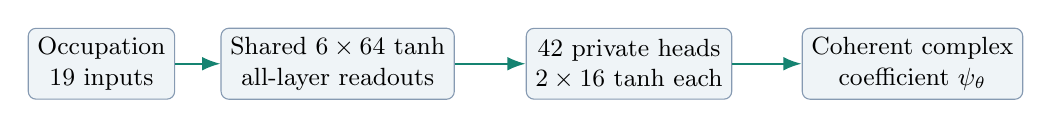
\begin{tikzpicture}[>=Latex,
box/.style={draw=blue!60,fill=pale,rounded corners=1mm,align=center,minimum height=.9cm,font=\small}]
\node[box] (in) at (0,0) {Occupation\\19 inputs};
\node[box] (base) at (3.0,0) {Shared $6\times64$ tanh\\all-layer readouts};
\node[box] (heads) at (6.7,0) {42 private heads\\$2\times16$ tanh each};
\node[box] (out) at (10.3,0) {Coherent complex\\coefficient $\psi_\theta$};
\draw[->,thick,teal] (in)--(base);
\draw[->,thick,teal] (base)--(heads);
\draw[->,thick,teal] (heads)--(out);
\end{tikzpicture}
\end{center}
\small
$\chi_s=1+r_s+i\,t_s$ uses two real outputs; $q_s=\operatorname{softmax}(z)_s$.
Each private head receives concatenated features from all six layers.\par\medskip
\textbf{294,464 real parameters}, including the 22,850-parameter shared base.
\take{Heads are learned angular features, not exact sector projectors or ED wavefunctions.}
\src{learned\_sector\_nonlinear\_model.py. All $W,b,R$, private-head weights and mixing logits are trained. The base alone has log magnitude/phase outputs; the complete coefficient includes coherent interference between heads.}
\end{frame}

% 13
\begin{frame}{Current sampling and solver settings}
\begin{columns}[T,onlytextwidth]
\column{.49\textwidth}
\textbf{Generate a weighted operator batch}\par\medskip
\small\renewcommand{\arraystretch}{1.12}
\begin{tabular}{@{}ll@{}}\toprule
Candidate pool & 512 valid uniform $M=0$ rows\\
Selected roots & 128 draws, with replacement\\
Selection & geometry + residual priority\\
Exploration & 20\% uniform pool component\\
Inverse selection & $\widetilde w_i=1/(512\pi_i)$\\
$H$ connections & 8 stochastic draws/root\\
$L_+$ outputs & 128 independent $M=1$ rows\\\bottomrule
\end{tabular}
\par\medskip
No physical temperature is introduced. Numerator and denominator use compatible importance weights.
\column{.47\textwidth}
\textbf{Stabilize the SPRING direction}\par\medskip
\small\renewcommand{\arraystretch}{1.12}
\begin{tabular}{@{}ll@{}}\toprule
Nominal $\eta$ & 0.001\\
Damping $\delta$ & 0.1\\
Direction memory $\mu$ & 0.9\\
Parameter radius & $r=0.015$\\
Augmented-state radius & 0.01\\
CG ceiling / tolerance & $1024\,/\,10^{-6}$\\
Held-out guard & every 50 attempts\\\bottomrule
\end{tabular}
\par\medskip
The cap and backtracking determine the actual step. The latest median $\alpha$ is $3.045\times10^{-4}$.
\end{columns}
\take{Candidate pool, selected batch, operator connections and update count are different computational budgets.}
\src{third10k config and metrics. $\sqrt{C_{\rm cap}}=0.015$; this cap is unrelated to conserved operator $C$. A typical batch has 99 distinct roots; median importance ESS is 42.09/128. Full sector is used only in frozen evaluation.}
\end{frame}

\section{Exact benchmarks and saved comparisons}
% 14
\begin{frame}{Ising validates the gradient and SPRING implementation}
\[
H_{\rm I}=-J\sum_i Z_iZ_{i+1}-h\sum_iX_i,\qquad N=6,\quad J=h=1.
\]
\begin{columns}[T,onlytextwidth]
\column{.67\textwidth}
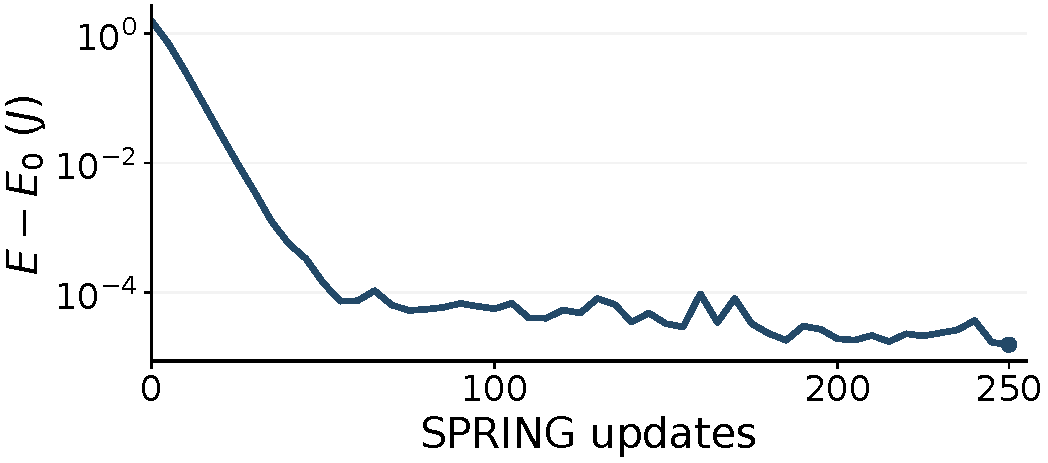
\includegraphics[width=\linewidth,height=3.7cm,keepaspectratio]{slide_ising.pdf}
\column{.30\textwidth}
\small
\textbf{64 configurations}\par
Positive even-parity RBM; 12 hidden units, 73 parameters.\par\medskip
\textbf{After 250 updates}
\[
E-E_0=1.576\times10^{-5}J
\]
\[
\fidelity=99.999857\%
\]
\[
\operatorname{Var}(H)=2.054\times10^{-4}J^2.
\]
$E_0/J=-7.727406610$.
\end{columns}
\take{Exact draws and full-basis checks validate the energy gradient before fermionic tests.}
\src{Retained SPRING\_Ising\_test result. Batch128, $\eta=.05$, damping .001, $\mu=.9$, radius .1; autodiff/energy-gradient discrepancy $1.94\times10^{-15}$. This is an implementation check, not a matched FQHE benchmark.}
\end{frame}

% 15
\begin{frame}{Matched short test: symmetry improves before physical energy}
\small Same mixed $h$, same source at 16k, same 294,464 parameters, $B=32$, pool128; \textbf{1,000 added attempts per arm}.
\begin{center}
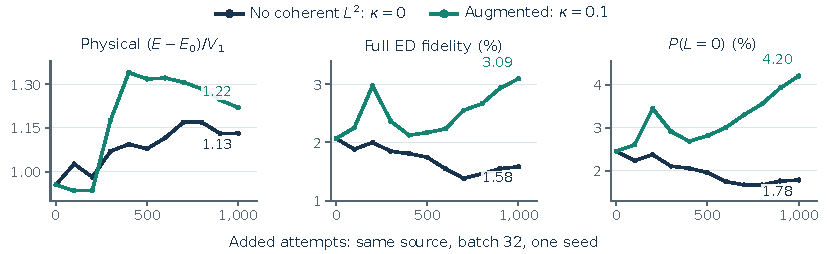
\includegraphics[width=.98\textwidth,height=3.9cm,keepaspectratio]{constraint_matched_short.pdf}
\end{center}
\take{Adding $\kappa=0.1$ improves ED fidelity and $L=0$ weight, but the physical energy is higher after this short test.}
\src{ne7\_angular\_time01\_matched1k and the identical reused $\kappa=0$ control. Both retain the same angular-head auxiliary loss, initial parameters, memory and RNG states. One seed; no confining potential. Comparison manifest verifies the matched source and inputs.}
\end{frame}

% 16
\begin{frame}{Long training gives a much better same-H ground-state approximation}
\small Same $N_e=7$, mixed Hamiltonian, no confining potential, 294,464-parameter angular-head architecture.
\par\medskip
\renewcommand{\arraystretch}{1.45}
\begin{tabular}{@{}L{.29\textwidth}rrrr@{}}
\toprule
Saved state & $E/V_1$ & $(E-E_0)/V_1$ & Full fidelity & $P(L=0)$\\\midrule
No coherent $L^2$, 16k & 7.199291 & 0.954523 & 2.066\% & 2.451\%\\
No coherent $L^2$, 17k & 7.376361 & 1.131592 & 1.582\% & 1.780\%\\
$\kappa=0.1$, latest 54k & \textbf{6.404269} & \textbf{0.159501} & \textbf{77.817\%} & \textbf{82.411\%}\\
ED ground & 6.244768 & 0 & 100\% & 100\%\\\bottomrule
\end{tabular}
\par\medskip
\begin{columns}[T,onlytextwidth]
\column{.49\textwidth}
\begin{block}{Observed improvement}
\small Relative to the 16k no-coherent-penalty state, energy excess falls by 83.3\% and full ED fidelity rises by 75.8 percentage points.
\end{block}
\column{.47\textwidth}
\begin{block}{Comparison scope}
\small Historical budgets differ: latest uses more attempts, $B=128$/pool512, revised anchors/guard and CG1024. This is not an isolated causal estimate of the $L^2$ term.
\end{block}
\end{columns}
\src{Audited no-coherent-penalty source at abs16000 and matched control at17000; latest third10k endpoint at54000. Same head auxiliary weight $\gamma=1$. The matched short test on slide15 is the controlled comparison.}
\end{frame}

% 17
\begin{frame}{At fixed $\kappa=0.1$, continued training improves the state}
\small Retained batch128 sequence, absolute attempts 19k--54k; pool512 and the same physical Hamiltonian throughout.
\begin{center}
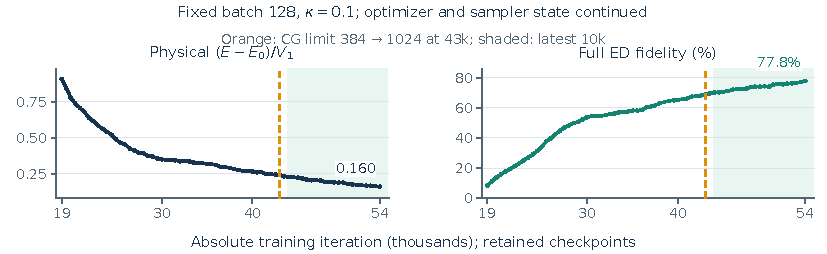
\includegraphics[width=.98\textwidth,height=4.0cm,keepaspectratio]{constraint_long_training.pdf}
\end{center}
\take{The latest 10k lowers energy error by 29.6\%: $0.22654\to0.15950\,V_1$; fidelity rises $70.18\%\to77.82\%$.}
\src{Stitched hash-verified frozen checkpoints; original tail after the failed solve is excluded from the retained path. At absolute43k, CG ceiling increased384 to1024; tolerance, physics and loss weights stayed fixed. These are continuation curves, not matched optimizer timings.}
\end{frame}

% 18
\begin{frame}{What remains inaccurate at the latest checkpoint?}
\begin{columns}[T,onlytextwidth]
\column{.48\textwidth}
\textbf{Complete-sector physical diagnostics}\par\medskip
\small\renewcommand{\arraystretch}{1.35}
\begin{tabular}{@{}lr@{}}\toprule
$E-E_0$ & $0.159501\,V_1$\\
$\operatorname{Var}(H)$ & $0.136171\,V_1^2$\\
Full ED fidelity & $77.817\%$\\
$P(L=0)$ & $82.411\%$\\
$\langle L^2\rangle/\hbar^2$ & $1.980676$\\
Conditional $L=0$ fidelity & $94.426\%$\\\bottomrule
\end{tabular}
\column{.48\textwidth}
\textbf{Decompose the remaining energy error}\par
\[
\|\Psi\|=1,\quad\Psi=\Psi_0+\Psi_\perp,\qquad
\Psi_0=P_{L=0}\Psi,
\]
\[
E-E_0=
\underbrace{0.044090}_{L=0}
+\underbrace{0.115410}_{L>0}\quad[V_1].
\]
\small Cross term vanishes because $[H,L^2]=0$.\par\medskip
\textbf{72.36\% of remaining error comes from outside $L=0$.} Shape error inside $L=0$ also remains.
\end{columns}
\take{Conditional projected accuracy is not the accuracy of the unprojected neural state.}
\src{third10k independent full-sector evaluation and separate NumPy/SciPy recomputation. One seed, finite budget, nonzero variance; no exact convergence or universal speedup is claimed. The projector is used here for diagnostics only.}
\end{frame}

\section{Generalization and conditions}
% 19
\begin{frame}{General $H+\lambda C$: preserve the target under stated conditions}
\[
[H,C]=0,\qquad H\ket a=E_a\ket a,\quad C\ket a=c_a\ket a
\quad\Longrightarrow\quad
(H+\lambda C)\ket a=(E_a+\lambda c_a)\ket a.
\]
\begin{columns}[T,onlytextwidth]
\column{.49\textwidth}
\begin{block}{Always true for commuting Hermitian operators}
\small A common eigenbasis exists.\par\medskip
Within a fixed $c$ sector, energy differences are unchanged:
\[
E_b^\lambda-E_a^\lambda=E_b-E_a.
\]
\end{block}
\column{.47\textwidth}
\begin{block}{Sufficient to keep the original ground state}
\small If $C\geq0$, $C\ket{\Psi_0}=0$, and $\lambda\geq0$, then
\[
E_a^\lambda-E_0=(E_a-E_0)+\lambda c_a\geq0.
\]
Unwanted sectors receive extra decay in imaginary time.
\end{block}
\end{columns}
\take{Commutation alone does not preserve global energy ordering. Excited states in different sectors may reorder.}
\src{For this benchmark, ED verifies $L_0=0$ and $C=K=L^2/\hbar^2\geq0$. A state with total $L$ gains $\kappa L(L+1)$ in $h_\kappa$. Symmetry penalties predate this project; see Kuroiwa--Nakagawa [7].}
\end{frame}

% 20
\begin{frame}{A reusable conserved-operator SPRING workflow}
\begin{center}
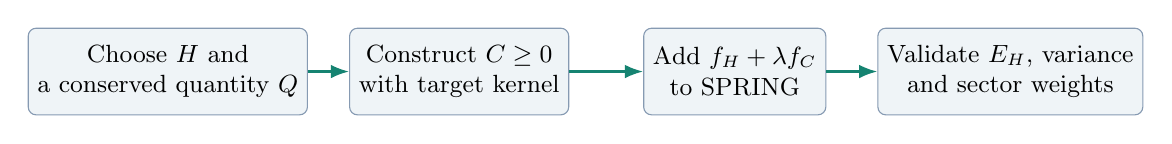
\begin{tikzpicture}[>=Latex,
box/.style={draw=blue!60,fill=pale,rounded corners=1mm,align=center,minimum height=1.1cm,font=\small}]
\node[box] (physics) at (0,0) {Choose $H$ and\\a conserved quantity $Q$};
\node[box] (penalty) at (3.7,0) {Construct $C\geq0$\\with target kernel};
\node[box] (force) at (7.2,0) {Add $f_H+\lambda f_C$\\to SPRING};
\node[box] (check) at (10.7,0) {Validate $E_H$, variance\\and sector weights};
\draw[->,thick,teal] (physics)--(penalty);
\draw[->,thick,teal] (penalty)--(force);
\draw[->,thick,teal] (force)--(check);
\end{tikzpicture}
\end{center}
\begin{itemize}\setlength\itemsep{7pt}
\item Example: $C=(Q-q_\star)^2$ for charge, spin component or another conserved label.
\item Verify the target-sector condition; an incorrect choice can bias the state away from the physical ground.
\item If $Q$ is already fixed exactly in the representation, this $C$ is constant and supplies no extra tangent force.
\item Next decisive test: equal-budget $\kappa=0$ versus $\kappa>0$ with the current batch128 model, plus sampling/solver diagnostics.
\end{itemize}
\take{Use symmetry to reshape unwanted-sector decay while evaluating success with the original physical Hamiltonian.}
\src{Current evidence: successful implementation and improved saved ground-state approximation; matched short test shows a tradeoff. Long-run benefit of the constraint alone still needs an equal-budget ablation.}
\end{frame}

\appendix
\section{Technical and reference backup}
% 21
\begin{frame}{Backup: normalized-state tangent derivation}
\small For a normalized neural state and Hermitian $F=H+\lambda C$,
\[
\frac{e^{-\tau F}\ket\Psi}{\|e^{-\tau F}\Psi\|}
=\ket\Psi-\tau(F-\langle F\rangle)\ket\Psi+O(\tau^2).
\]
Remove the component parallel to $\Psi$:
\[
\delta\Psi_\theta(\nn)=\psi_\theta(\nn)
\sum_j\delta O_j(\nn)\,\Delta\theta_j,\qquad
\delta O_j=O_j-\langle O_j\rangle.
\]
\[
\min_{\Delta\theta\in\R^P}
\left\|A\Delta\theta+\tau(e_H+\lambda e_C)\right\|^2.
\]
\[
f_H=\Re\langle\delta O^*\delta E_{\rm loc}\rangle,\qquad
f_C=\Re\langle\delta O^*\delta C_{\rm loc}\rangle,\qquad
\tfrac12\nabla(E_H+\lambda\langle C\rangle)=f_H+\lambda f_C.
\]
\take{The added force is an operator fluctuation in tangent space, not a configuration-space angular label.}
\src{Exact identities assume full-state expectations and real trainable parameters. Finite sampled ratios, stochastic H connections and the head auxiliary term require the implemented autodiff equation.}
\end{frame}

% 22
\begin{frame}{Backup: exactly when is the global ordering preserved?}
\[
\text{For }E_a<E_b:\qquad
E_a+\lambda c_a<E_b+\lambda c_b
\ \ \Longleftrightarrow\ \
(E_b-E_a)+\lambda(c_b-c_a)>0.
\]
\small For $\lambda\geq0$, any pair with $c_a>c_b$ requires
\[
\lambda<\frac{E_b-E_a}{c_a-c_b}.
\]
A nondecreasing $c_a$ as $E_a$ increases is another sufficient condition.
\begin{columns}[T,onlytextwidth]
\column{.49\textwidth}
\begin{block}{Commuting counterexample}
\small $H=\operatorname{diag}(0,1)$,\quad $C=\operatorname{diag}(2,0)$.\par\medskip
They commute, but $\lambda=1$ gives energies $(2,1)$ and changes the ground state.
\end{block}
\column{.47\textwidth}
\begin{block}{Ground preserved, excited levels reordered}
\small $H=\operatorname{diag}(0,1,2)$,\quad $C=\operatorname{diag}(0,2,0)$.\par\medskip
At $\lambda=1$, energies $(0,3,2)$ retain the ground but reverse two excited levels.
\end{block}
\end{columns}
\src{Ordering refers to eigenvalues of the generator $H+\lambda C$. The propagator $e^{-\tau(H+\lambda C)}$ preserves the joint eigenvectors and changes their decay factors; it is not generally isospectral to $H$.}
\end{frame}

% 23
\begin{frame}{Backup: head auxiliary loss and the actual projective metric}
\small Let $\Psi=\sum_s q_s\Psi_s$ and $k_s=L_s(L_s+1)$ for the 42 allowed angular labels. The retained auxiliary term is
\[
\mathcal A_{\rm heads}=
\frac1{42}\sum_s
\frac{\|(K-k_s)\Psi_s\|^2}{630^2\,\|\Psi_s\|^2}.
\]
For normalized physical state $\widehat\Psi$ and heads $\widehat\Psi_s$,
\[
(G_{\rm aug})_{ij}=
\Re\langle\partial_i\widehat\Psi|
(1-\ket{\widehat\Psi}\bra{\widehat\Psi})
|\partial_j\widehat\Psi\rangle
+\frac1{42}\sum_s
\Re\langle\partial_i\widehat\Psi_s|
(1-\ket{\widehat\Psi_s}\bra{\widehat\Psi_s})
|\partial_j\widehat\Psi_s\rangle.
\]
\[
f=\tfrac12\nabla\!\left[E_h+\gamma\mathcal A_{\rm heads}
+\kappa\langle K\rangle\right],\quad
(G_{\rm aug}+\delta I)d=f+\delta\mu d_{\rm prev}.
\]
\take{Head residual training and the coherent $L^2$ force are distinct. Neither is a dense angular projector.}
\src{Full-state formulas above use weighted sampled counterparts in code. 630 is the existing dimensionless head-residual scale $N_eQ(Q+1)$, not the coherent penalty normalization. The $L^2$ term does not add new Gauss--Newton curvature to this metric.}
\end{frame}

% 24
\begin{frame}{Backup: comparison provenance and finite-batch limits}
\small\renewcommand{\arraystretch}{1.25}
\begin{tabular}{@{}L{.25\textwidth}L{.32\textwidth}L{.34\textwidth}@{}}\toprule
Comparison & Shared controls & Remaining differences / scope\\\midrule
Matched 1k, $\kappa=0$ vs $0.1$
& Same source, parameters, memory, RNGs, mixed $h$, head loss; batch32/pool128
& Only coherent penalty weight differs; one seed, short budget.\\
Historical 16k vs latest54k
& Same mixed $h$, 294,464-parameter architecture, head auxiliary weight
& More updates; batch32 to128, pool128 to512; guard/anchors/CG budget differ.\\
Latest 10k continuation
& Full optimizer/sampler restore, batch128, $\kappa=.1$, CG1024
& Single continued trajectory; no new equal-budget control.\\\bottomrule
\end{tabular}
\par\medskip
\begin{itemize}\setlength\itemsep{4pt}
\item Finite self-normalized ratios/covariances are biased; sampled energy is not a variational bound.
\item Latest median root ESS is $42.09/128$; sampled physical energy is below ED on 3,726/10,000 attempts.
\item Full-state ED energy, fidelity, variance and sector weights are evaluated only after freezing each checkpoint.
\end{itemize}
\src{constraint\_comparison\_20261116.json:269 source artifacts verified. Latest independent audit:21states/10kattempts/200guards; maxCG920, no failure. Original archived recovery and discarded work remain documented.}
\end{frame}

% 25
\begin{frame}{References}
\footnotesize
\begin{enumerate}\setlength\itemsep{4pt}
\item F. D. M. Haldane, \emph{Fractional quantization of the Hall effect}, PRL 51,605 (1983). \href{https://doi.org/10.1103/PhysRevLett.51.605}{doi:10.1103/PhysRevLett.51.605}.
\item R. B. Laughlin, \emph{Anomalous quantum Hall effect}, PRL 50,1395 (1983). \href{https://doi.org/10.1103/PhysRevLett.50.1395}{doi:10.1103/PhysRevLett.50.1395}.
\item G. Carleo and M. Troyer, \emph{Solving the quantum many-body problem with artificial neural networks}, Science355,602 (2017). \href{https://arxiv.org/abs/1606.02318}{arXiv:1606.02318}.
\item A. Chen and M. Heyl, \emph{Empowering deep neural quantum states through efficient optimization}, Nature Physics20,1476 (2024). \href{https://arxiv.org/abs/2302.01941}{arXiv:2302.01941}.
\item G. Goldshlager, N. Abrahamsen and L. Lin, \emph{A Kaczmarz-inspired approach to accelerate the optimization of neural network wavefunctions}, JCP516,113351 (2024). \href{https://arxiv.org/abs/2401.10190}{arXiv:2401.10190}.
\item Y. Teng, D. D. Dai and L. Fu, \emph{Solving and visualizing fractional quantum Hall wavefunctions with neural network}, PRB111,205117 (2025). \href{https://arxiv.org/abs/2412.00618}{arXiv:2412.00618}.
\item K. Kuroiwa and Y. O. Nakagawa, \emph{Penalty methods for variational quantum eigensolver}, PRR3,013197 (2021). \href{https://doi.org/10.1103/PhysRevResearch.3.013197}{doi:10.1103/PhysRevResearch.3.013197}.
\end{enumerate}
\src{[5] is the original SPRING optimizer; [6] is the real-space FQH/FNN paper and differs from this strictly LLL occupation-space model. Conserved-operator penalties are established methodology; this project implements and tests their coupling to SPRING.}
\end{frame}
\end{document}
